\documentclass[9pt,a4paper,twocolumn]{article}
\usepackage{fullpage, graphicx, url, enumitem, parskip, eurosym}
\usepackage[utf8]{inputenc}

\newlist{tip}{itemize}{1}
\setlist[tip,1]{
  leftmargin=\dimexpr1.2cm+\labelsep\relax,
  label={\smash{\raisebox{-0.6\height}{
\includegraphics[width=1.5cm]{images/icons/tip.png}}}}
}

\newlist{arrow_red}{itemize}{1}
\setlist[arrow_red,1]{
  leftmargin=\dimexpr0.5cm+\labelsep\relax,
  label={\smash{\raisebox{-0.3\height}{
\includegraphics[width=0.5cm]{images/icons/arrow_red.png}}}}
}

\newlist{arrow_yellow}{itemize}{1}
\setlist[arrow_yellow,1]{
  leftmargin=\dimexpr0.5cm+\labelsep\relax,
  label={\smash{\raisebox{-0.3\height}{
\includegraphics[width=0.5cm]{images/icons/arrow_yellow.png}}}}
}

\newlist{arrow_blue}{itemize}{1}
\setlist[arrow_blue,1]{
  leftmargin=\dimexpr0.5cm+\labelsep\relax,
  label={\smash{\raisebox{-0.3\height}{
\includegraphics[width=0.5cm]{images/icons/arrow_blue.png}}}}
}

\newlist{arrow_green}{itemize}{1}
\setlist[arrow_green,1]{
  leftmargin=\dimexpr0.5cm+\labelsep\relax,
  label={\smash{\raisebox{-0.3\height}{
\includegraphics[width=0.5cm]{images/icons/arrow_green.png}}}}
}

\newlist{arrow_pink}{itemize}{1}
\setlist[arrow_pink,1]{
  leftmargin=\dimexpr0.5cm+\labelsep\relax,
  label={\smash{\raisebox{-0.3\height}{
\includegraphics[width=0.5cm]{images/icons/arrow_pink.png}}}}
}

\setlength{\parindent}{0em}
\setlength{\parskip}{1em}

\begin{document}


\includegraphics[width=\linewidth]{images/logo.png}
SkySight (https://skysight.io/) ist ein interaktives Wettervorhersageprogramm, entwickelt von einem Team von Meteorologen und Segelflug-Weltmeistern. Es kombiniert die neusten Vorhersage-Technologien mit einer intuitiven Benutzeroberfläche, und stellt hochauflösende Vorhersagen und leistungsstarke Streckenplanungsprogramme zur Verfügung. Das Programm steht für Vorhersagen in einem Großteil der Welt zur Verfügung und ist für 79 {\euro} pro Jahr (zum Zeitpunkt der Verfassung) erhältlich.


 
\subsection*{Lokale Vorhersagen}
Mit SkySight ist es sehr einfach die Wetterlage zu verstehen. Thermik, Welle, Konvergenz und Hangauftrieb werden mit leicht zu verstehenden farbkodierten Karten visualisiert. 

Der einfachste Weg, sich die Vorhersage anzeigen zu lassen, ist die \textbf{Punktvorhersage}. Diese zeigt Thermik, Wolkenbedeckung und signifikantes Wetter in einer praktischen Zusammenfassung an.

Da komplexe lokale Effekte signifikanten Einfluss auf die Punktvorhersage an einem genauen Ort, nicht aber an den herumliegenden Orten haben können, wird empfohlen, die Punktvorhersage an mehreren Orten um den Flugplatz aufzurufen.


\subsection*{Streckenplanung}
Streckenplanung stellt sich oft als kompliziert dar, mit sich ändernden thermischen Konditionen, Wolkenbedeckung, Überentwicklung, Wind, Luftraum, Konvergenzen, Welle und vielen anderen Faktoren.

SkySight versucht die Wahl der Strecke so einfach wie möglich zu machen:

\begin{enumerate}
  \item Die \textbf{Thermikhöhe} und \textbf{Thermikstärke} über den Tagesverlauf hilft Ihnen dabei, sich eine Übersicht über den Bereich, in dem der Flug stattfinden soll, zu verschaffen.
  \item Schätzen Sie die Startzeit ab und berechnen Sie das Zeitfenster für den Flug. Die \textbf{Potenzielle Flugdistanz} kann als Richtlinie für die maximale Strecke genommen werden. 
    \item Mit der \textbf{Cu Basis} Funktion wird visualisiert, wo Cumuluswolken erwartet werden. Graue Flächen zeigen mögliche kleine Wolkenformationen oder einen gewissen Grad der Ungewissheit an.
\item Die \textbf{Cu vertikale Ausdehnung} zeigt die Art der Thermik an – positive Werte bedeuten Cumuluswolken, negative Werte bedeuten Blauthermik.
  \item Um die Windrichtung zu bestimmen, benutzen Sie die \textbf{Wind Obergrenze Grenzschicht} Funktion. Wenn möglich, bietet es sich an, die Schenkel an die Windrichtung anzupassen.
\item Die \textbf{Konvergenz} Funktion zeigt mögliche Konvergenzlinien an, von denen während des Fluges Gebrauch gemacht werden kann. Lange orangene oder rote Linien sind ideal.
  \item \textbf{Wolkenbedeckung}, \textbf{Überentwicklung} und \textbf{CAPE/Sturm} gibt Ihnen Aufschluss über unerwartete Wetterbedingungen.
\item Wählen Sie die \textbf{Satellitenansicht} aus, um zu bestätigen, dass sich die momentanen Wetterverhältnisse mit der Vorhersage abdecken. Der direkte Vergleich lässt sich leicht machen, indem das Satellitenbild mit der \textbf{Vorhergesagten Satellitenansicht} verglichen wird.
  \item Wenn Sie all diese Informationen in Betracht gezogen haben, können Sie die Strecke mithilfe der \textbf{Routenvorhersage} auswählen.
  \item Bestätigen Sie Ihr Verständnis der Vorhersage, indem Sie sich die \textbf{Punktvorhersage} an verschiedenen Stellen der Strecke anschauen. Damit stellen Sie sicher, dass Sie die gesamten Wetterbedingungen über den Tag in Betracht gezogen haben.
\item Eine noch detaillierte Analyse können Sie mit Hilfe des \textbf{Vertikalprofiles} und des \textbf{Punkt-Winddiagrammes} durchführen.
  \item Fliegen Sie los! Benutzen Sie die \textbf{IGC Upload} Funktion am Ende des Tages um Ihren Flug zu analysieren.
\end{enumerate}

\subsection*{Interaktive Funktionen von SkySight}
Interaktive Funktionen von SkySight
\begin{enumerate}
  \item Wählen Sie die gewünschte Funktion im Seitenmenü aus.
  \item Klicken Sie an den Ort, für welchen die Vorhersage angezeigt werden soll.
  \item Definieren Sie bei der Routen- und Wellenvorhersage die Strecke, indem Sie erneut auf die Karte klicken.
  \item Wenn Sie das Zeitfenster ändern möchten, können Sie die rote Start und End-Zeit an die gewünschte Zeit anpassen.
  \item Um das Fenster zu schließen, klicken Sie 
\includegraphics[height=12pt]{images/icons/exit.png}.
\end{enumerate}
\subsubsection*{
\includegraphics[height=15pt]{images/icons/skew-t.png} Vertikalprofil}
Das Skew-T log-P Diagramm wird dazu verwendet, die konvektive Grenzschicht, Konditionen im oberen Bereich der Atmosphäre, sowie Sturmpotenzial und Wind zu bestimmen. SkySight generiert ein leicht zu verstehendes Diagramm für jeden beliebigen Ort auf der Karte.

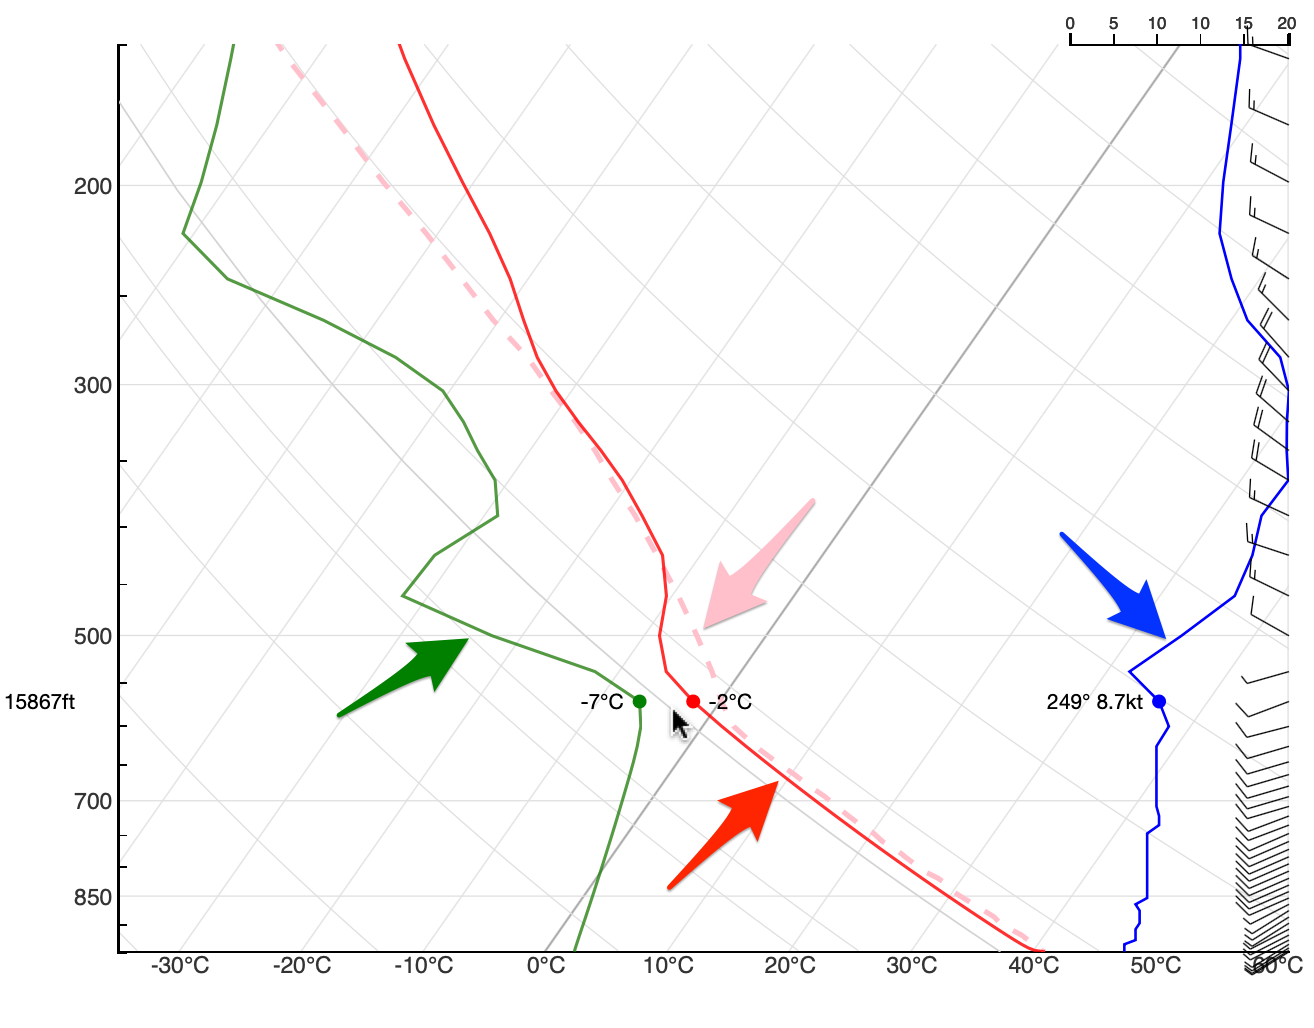
\includegraphics[width=\linewidth]{images/skew-t.png}

\begin{arrow_red}
\item \textbf{Temperaturkurve} Die vorhergesagte Temperatur mit sich ändernder Höhe 
\end{arrow_red}
\begin{arrow_green}
\item \textbf{Taupunktkurve} Der vorhergesagte Taupunkt mit sich ändernder Höhe
\end{arrow_green}
\begin{arrow_blue}
\item \textbf{Windstärke} Die vorhergesagte Windstärke mit sich ändernder Höhe 
\end{arrow_blue}
\begin{arrow_pink}
\item \textbf{Virtuelles Luftpaket} Ein simuliertes Paket warmer Luft, welches sich durch die Grenzschicht bewegt. Dieses wird genutzt, um die Wahrscheinlichkeit von Sturmentwicklungen vorherzusagen. 
\end{arrow_pink}
\subsubsection*{
\includegraphics[height=15pt]{images/icons/point_forecast.png} Punktvorhersage}

Mit der Punktvorhersage werden die Wetterverhältnisse des gesamten Tages schnell und übersichtlich angezeigt. Wolkenbedeckung, thermische Aktivität und Temperaturen werden visualisiert sowie als Werte dargestellt.



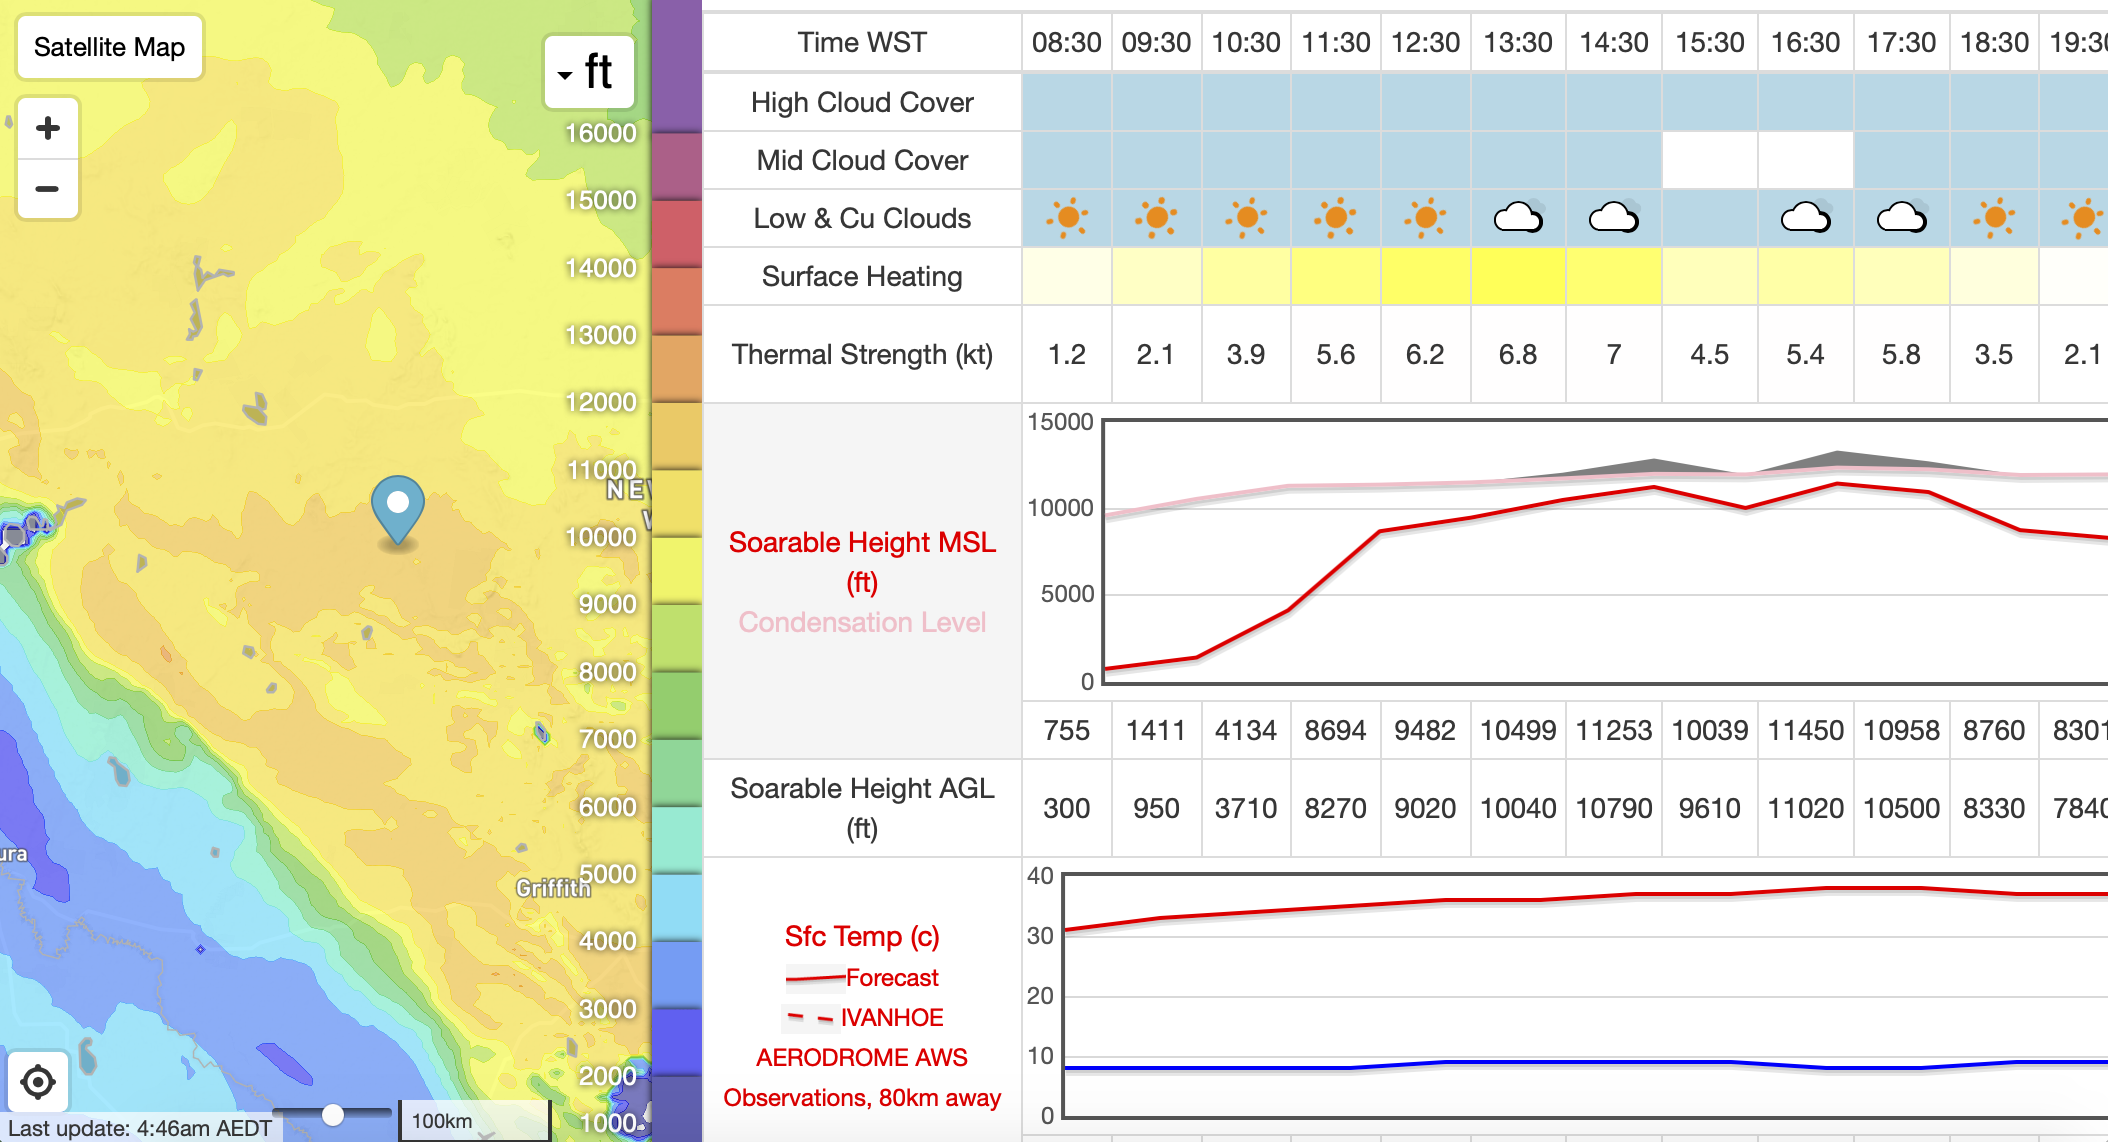
\includegraphics[width=\linewidth]{images/point_forecast.png}

Die Wolkenbedeckung wird in der oberen Reihe mit Hilfe eines Farbverlaufes dargestellt. Blau zeigt klare Verhältnisse, weiß zeigt dünne Wolken und dunklere Grautöne dickere Wolken.

Die vertikale Ausdehnung der Cumuluswolken wird durch die grau ausgefüllte Fläche über dem Kondensationslevel angezeigt. Wenn keine graue Fläche zu sehen ist, bedeutet dies Blauthermik.

\subsubsection*{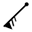
\includegraphics[height=15pt]{images/icons/windgram.png} Punkt-Winddiagramm}
Das Winddiagramm zeigt die Entwicklung des atmosphärischen Temperaturgradientens, der Temperatur, der relativen Feuchtigkeit und des Windes während des gesamten Tages zusammen mit der Höhe an einem bestimmten Ort. Diese Funktion ist praktisch, um die Inversionsschicht, Feuchtigkeitsschichten und Windgradienten darzustellen.

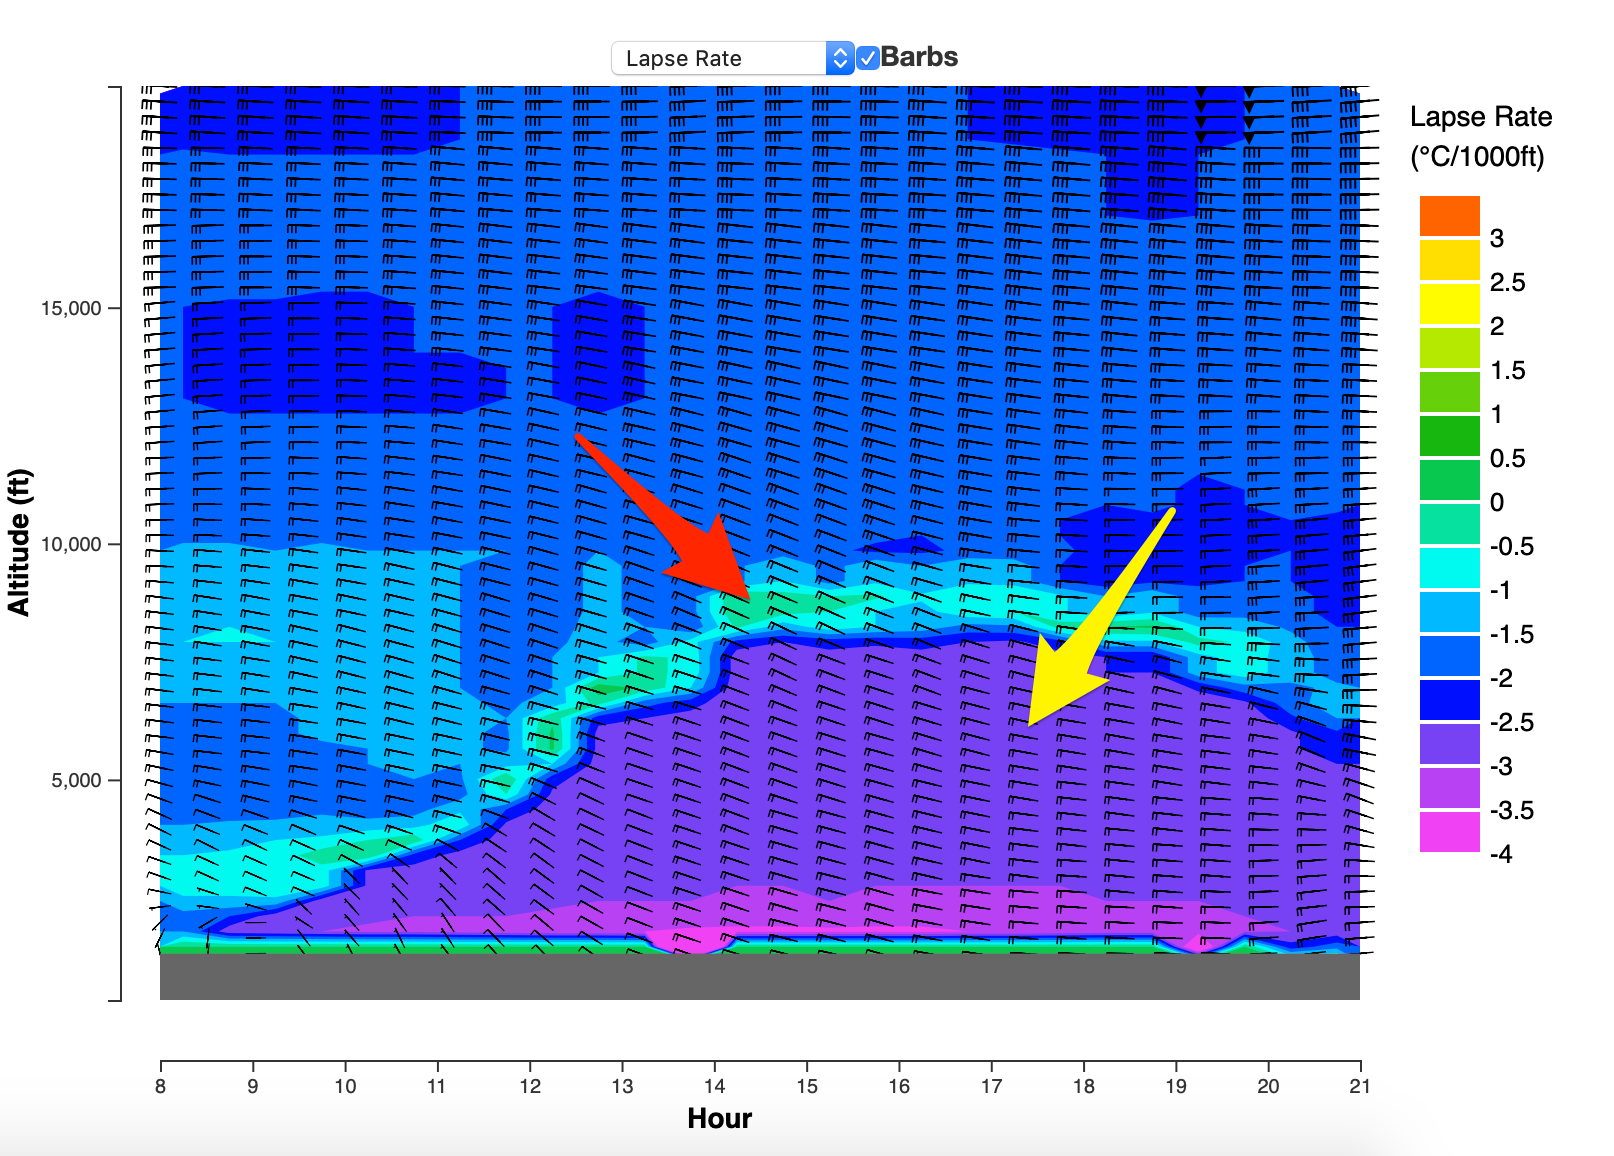
\includegraphics[width=\linewidth]{images/windgram_lapse_annot.png}
Hier wird mit Hilfe des atmosphärischen Temperaturgradienten ein typischer Flugtag gezeigt. Die Inversion (
\includegraphics[height=11pt]{images/icons/arrow_red.png}) steigt im Laufe des Tages und die konvektive Grenzschicht (
\includegraphics[height=11pt]{images/icons/arrow_yellow.png}) wird tiefer. 


\subsubsection*{
\includegraphics[height=15pt]{images/icons/route.png} Routenvorhersage}
Die Routenvorhersagefunktion berechnet die voraussichtliche Geschwindigkeit und fasst die vorhergesagten Konditionen im Verlauf der Strecke zusammen. Für Streckenplanung und Wettbewerbsflüge ist dies eine sehr hilfreiche Funktion. Die Tabelle rechts zeigt die vorhergesagte Geschwindigkeit zu verschiedenen Zeitpunkten an. Inf. bedeutet, dass die Strecke möglicherweise nicht zu schaffen ist. Die Wendepunkte können bewegt werden und somit ist es leicht, realistischere Strecken zu finden und die Startzeit zu optimieren. 
Möglicherweise müssen Sie die Punkte verschieben, wenn diese in Orten mit unfliegbaren Bedingungen liegen, um eine realistische Geschwindigkeit angezeigt zu bekommen.


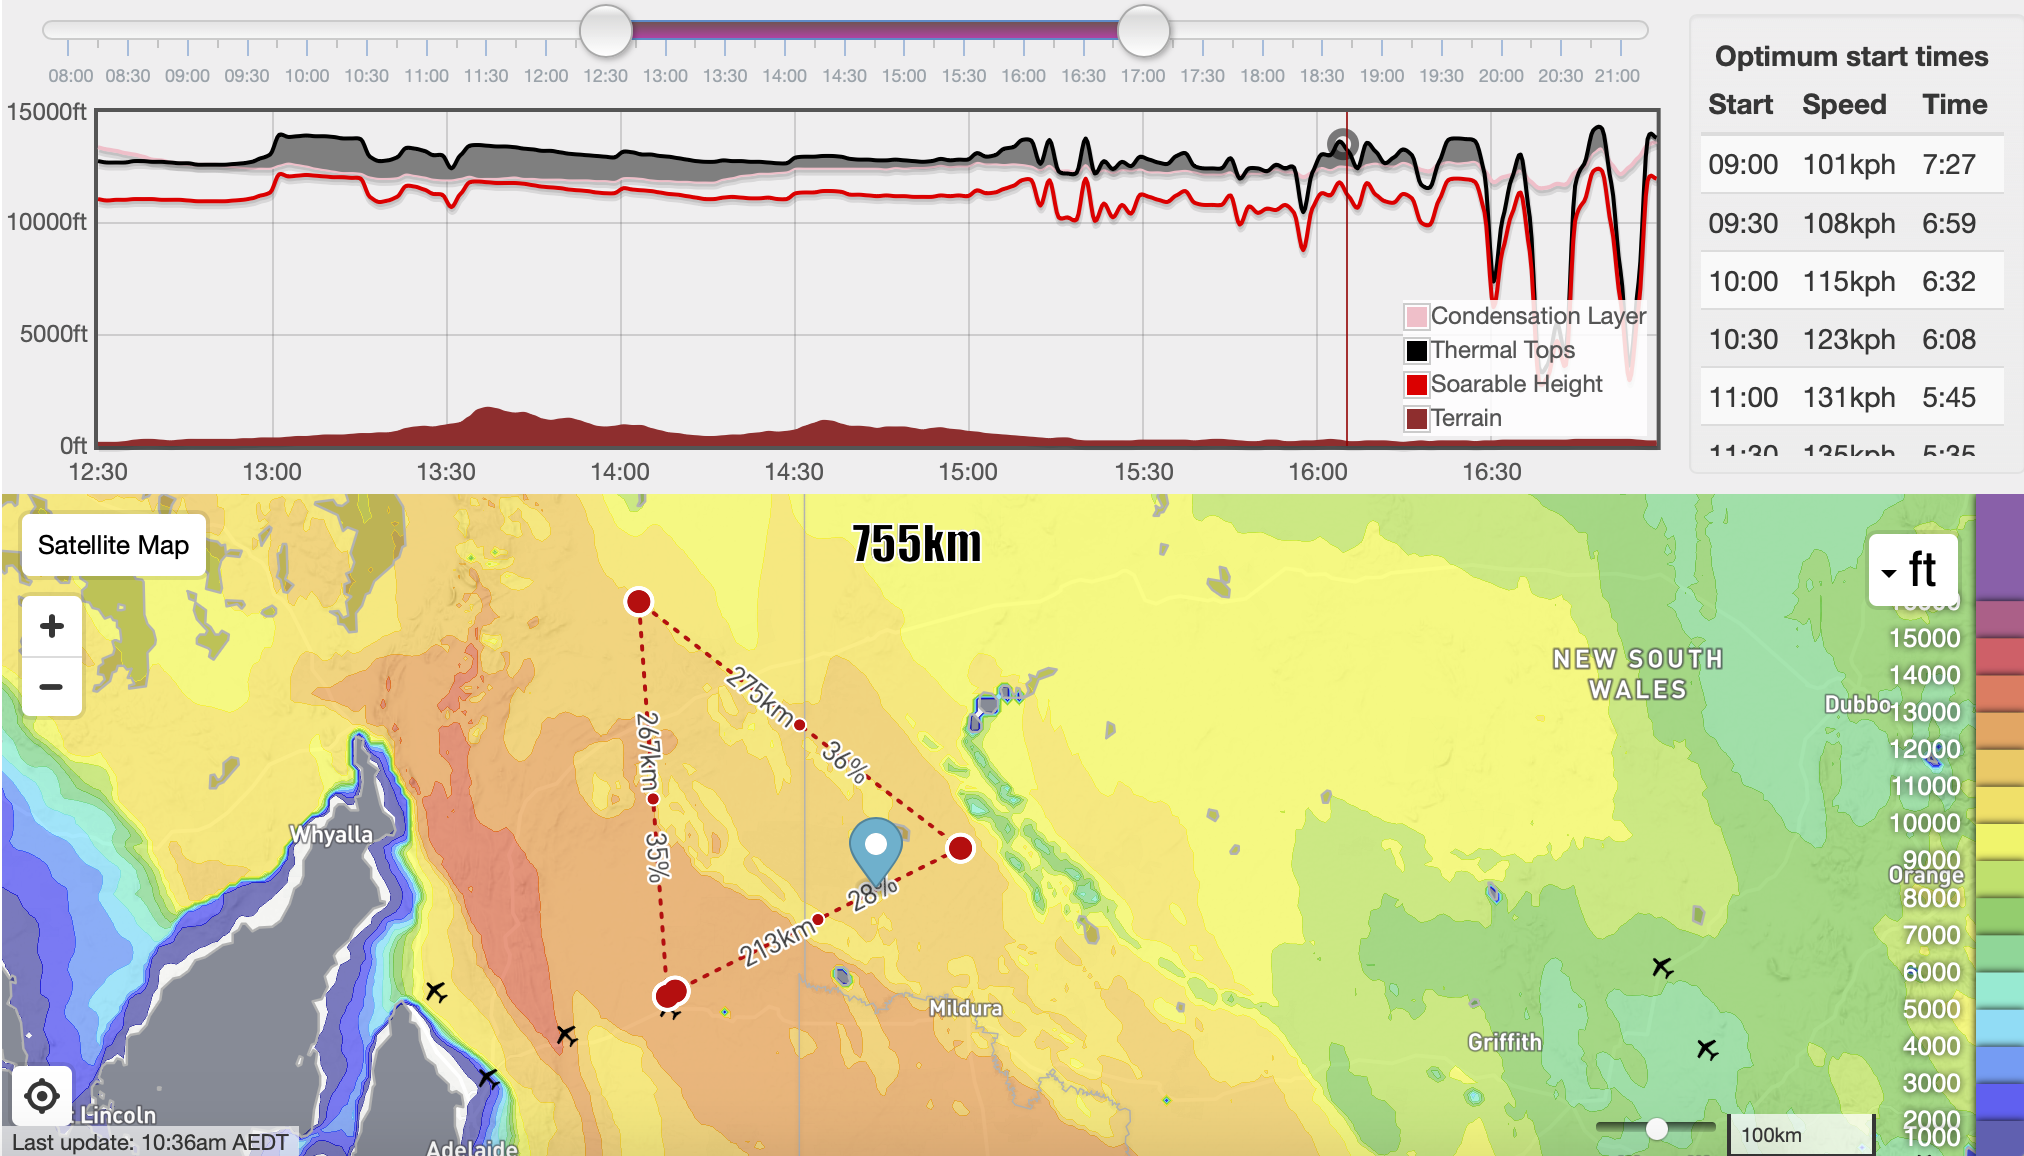
\includegraphics[width=\linewidth]{images/route.png}
\subsubsection*{
\includegraphics[height=15pt]{images/icons/wave.png} Wellenquerschnitt}
Der Wellenquerschnitt ermöglicht es, die Eigenschaften der Welle mit sich ändernder Höhe darzustellen. Es wird eine 2D Abbildung der Wellenvorhersage zwischen zwei Punkten dargestellt, mit der Höhe auf der vertikalen und Distanz zwischen zwei Punkten auf der horizontalen Are, sowie farbkodierter vertikaler Geschwindigkeit.

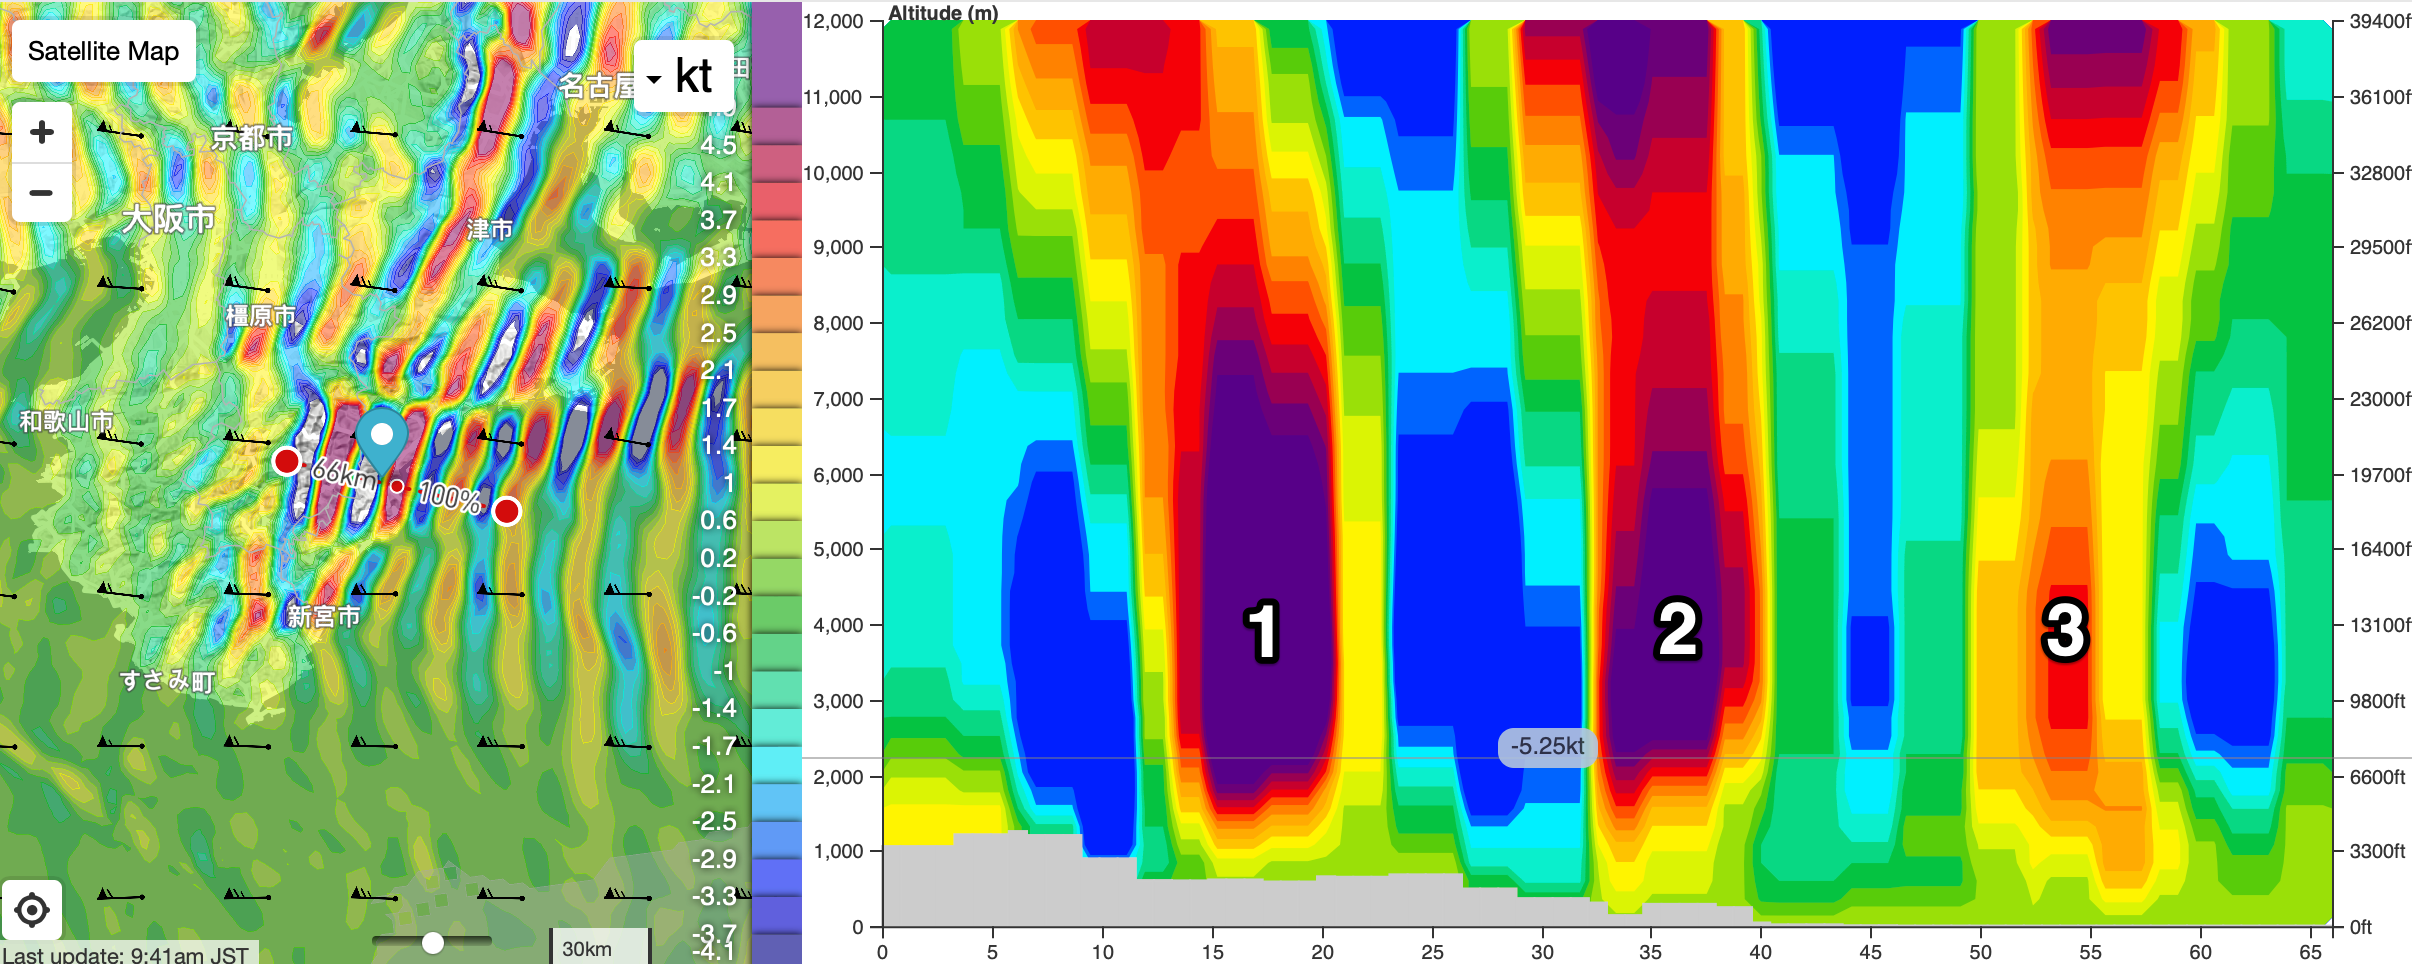
\includegraphics[width=\linewidth]{images/wave_x-section.png}

Die Abbildung zeigt einen Wellenquerschnitt durch die Japanischen Alpen. Regionen 1, 2 und 3 zeigen die ersten, zweiten und dritten Wellen. Rot und lila zeigt Auftrieb, blau Sinken an.


\subsubsection*{
\includegraphics[height=15pt]{images/icons/igc.png} IGC Upload}
SkySight kann dazu genutzt werden, im Nachhinein den Flug zu analysieren. Das hilft insbesondere dabei, Beobachtungen, die während des Fluges gemacht wurden zu bestätigen und die Entwicklung und Interpretation dieser in den SkySight Vorhersagen zu verstehen.

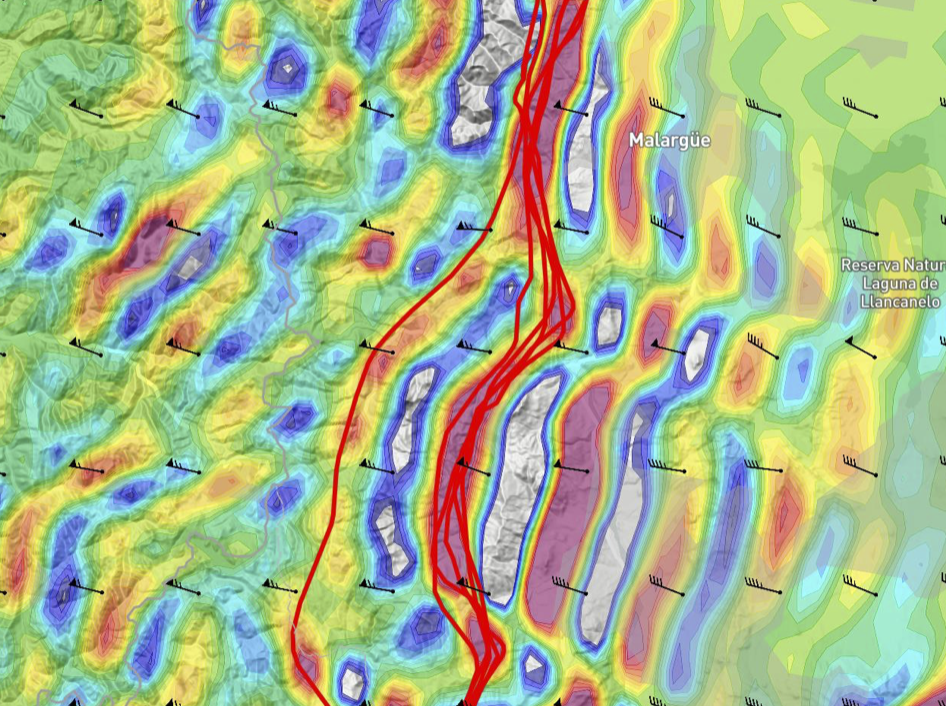
\includegraphics[width=\linewidth]{images/igc_upload.png}

\subsection*{Zugriff auf SkySight}
SkySight steht sowohl für Computer, als auch für mobile Geräte zur Verfügung. Einen kostenlosen Probezugang, sowie Abonnements sind auf \url{https://skysight.io/} verfügbar.

\end{document}
